\documentclass{standalone}
\usepackage{tikz}
\usetikzlibrary{patterns, positioning}


\begin{document}
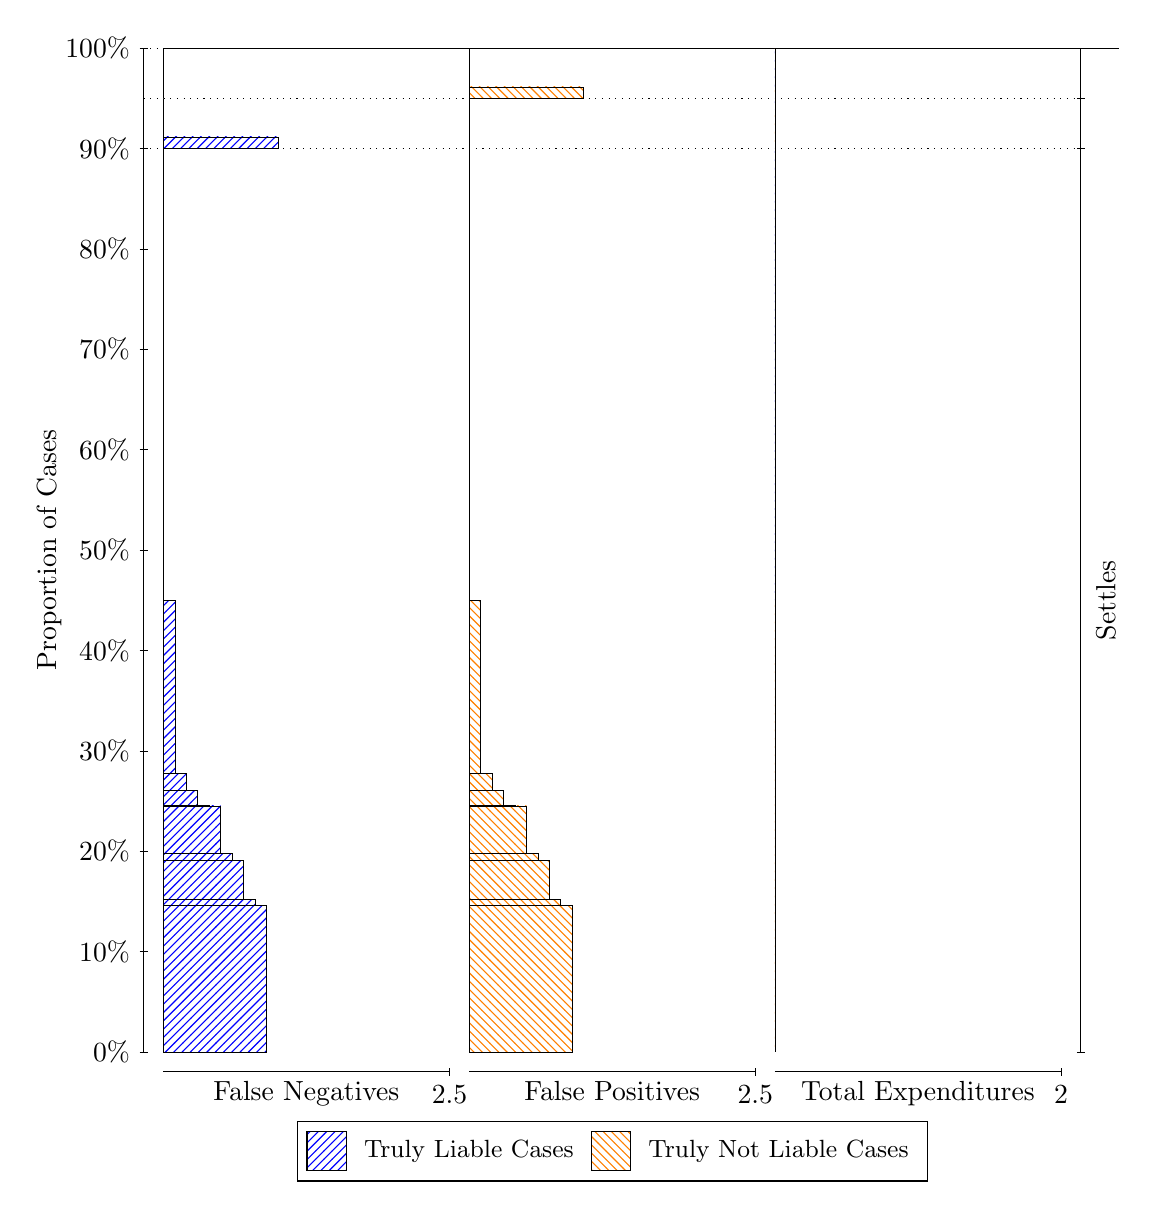
\begin{tikzpicture}
\draw[black, very thin] (1.5,1.75) -- (1.5,14.5);
\node[rotate=90, text=black, anchor=center] at (0.3, 8.125) {Proportion of Cases};
\draw[black, very thin] (1.45,1.75) -- (1.55,1.75);
\node[text=black, anchor=east] at (1.45, 1.75) {0\%};
\draw[black, very thin] (1.45,3.025) -- (1.55,3.025);
\node[text=black, anchor=east] at (1.45, 3.025) {10\%};
\draw[black, very thin] (1.45,4.3) -- (1.55,4.3);
\node[text=black, anchor=east] at (1.45, 4.3) {20\%};
\draw[black, very thin] (1.45,5.575) -- (1.55,5.575);
\node[text=black, anchor=east] at (1.45, 5.575) {30\%};
\draw[black, very thin] (1.45,6.85) -- (1.55,6.85);
\node[text=black, anchor=east] at (1.45, 6.85) {40\%};
\draw[black, very thin] (1.45,8.125) -- (1.55,8.125);
\node[text=black, anchor=east] at (1.45, 8.125) {50\%};
\draw[black, very thin] (1.45,9.4) -- (1.55,9.4);
\node[text=black, anchor=east] at (1.45, 9.4) {60\%};
\draw[black, very thin] (1.45,10.675) -- (1.55,10.675);
\node[text=black, anchor=east] at (1.45, 10.675) {70\%};
\draw[black, very thin] (1.45,11.95) -- (1.55,11.95);
\node[text=black, anchor=east] at (1.45, 11.95) {80\%};
\draw[black, very thin] (1.45,13.225) -- (1.55,13.225);
\node[text=black, anchor=east] at (1.45, 13.225) {90\%};
\draw[black, very thin] (1.45,14.5) -- (1.55,14.5);
\node[text=black, anchor=east] at (1.45, 14.5) {100\%};

\draw[black, very thin] (13.4,1.75) -- (13.4,14.5);
\draw[black, very thin] (13.35,1.75) -- (13.45,1.75);
\node[anchor=west] at (13.35, 1.75) {};
\draw[black, very thin] (13.35,13.226) -- (13.45,13.226);
\node[anchor=west] at (13.35, 13.226) {};
\draw[black, very thin] (13.35,13.861) -- (13.45,13.861);
\node[anchor=west] at (13.35, 13.861) {};
\draw[black, very thin] (13.35,14.496) -- (13.45,14.496);
\node[anchor=west] at (13.35, 14.496) {};
\draw[black, very thin] (13.35,14.498) -- (13.45,14.498);
\node[anchor=west] at (13.35, 14.498) {};
\draw[black, very thin] (13.35,14.5) -- (13.45,14.5);
\node[anchor=west] at (13.35, 14.5) {};

\draw[black, very thin, pattern color=blue, pattern=north east lines] (1.75,1.75) rectangle (3.058,3.6136);
\draw[black, very thin, pattern color=blue, pattern=north east lines] (1.75,3.6136) rectangle (2.9127,3.6921);
\draw[black, very thin, pattern color=blue, pattern=north east lines] (1.75,3.6921) rectangle (2.7673,4.1854);
\draw[black, very thin, pattern color=blue, pattern=north east lines] (1.75,4.1854) rectangle (2.622,4.2743);
\draw[black, very thin, pattern color=blue, pattern=north east lines] (1.75,4.2743) rectangle (2.4767,4.8757);
\draw[black, very thin, pattern color=blue, pattern=north east lines] (1.75,4.8757) rectangle (2.3313,4.886);
\draw[black, very thin, pattern color=blue, pattern=north east lines] (1.75,4.886) rectangle (2.186,5.0681);
\draw[black, very thin, pattern color=blue, pattern=north east lines] (1.75,5.0681) rectangle (2.0407,5.285);
\draw[black, very thin, pattern color=blue, pattern=north east lines] (1.75,5.285) rectangle (1.8953,7.4881);
\draw[black, very thin, pattern color=orange, pattern=north west lines] (1.75,7.4881) rectangle (1.75,13.226);
\draw[black, very thin, pattern color=blue, pattern=north east lines] (1.75,13.226) rectangle (3.2033,13.372);
\draw[black, very thin, pattern color=orange, pattern=north west lines] (1.75,13.372) rectangle (1.75,13.861);
\draw[black, very thin, pattern color=orange, pattern=north west lines] (1.75,13.861) rectangle (1.75,14.007);
\draw[black, very thin, pattern color=blue, pattern=north east lines] (1.75,14.007) rectangle (1.75,14.496);
\draw[black, very thin, pattern color=blue, pattern=north east lines] (1.75,14.496) rectangle (5.8193,14.497);
\draw[black, very thin, pattern color=orange, pattern=north west lines] (1.75,14.497) rectangle (1.75,14.498);
\draw[black, very thin, pattern color=blue, pattern=north east lines] (1.75,14.498) rectangle (2.622,14.499);
\draw[black, very thin, pattern color=orange, pattern=north west lines] (1.75,14.499) rectangle (1.75,14.5);
\draw[black, very thin, pattern color=orange, pattern=north west lines] (5.6333,1.75) rectangle (6.9413,3.6136);
\draw[black, very thin, pattern color=orange, pattern=north west lines] (5.6333,3.6136) rectangle (6.796,3.6921);
\draw[black, very thin, pattern color=orange, pattern=north west lines] (5.6333,3.6921) rectangle (6.6507,4.1855);
\draw[black, very thin, pattern color=orange, pattern=north west lines] (5.6333,4.1855) rectangle (6.5053,4.2744);
\draw[black, very thin, pattern color=orange, pattern=north west lines] (5.6333,4.2744) rectangle (6.36,4.8758);
\draw[black, very thin, pattern color=orange, pattern=north west lines] (5.6333,4.8758) rectangle (6.2147,4.8861);
\draw[black, very thin, pattern color=orange, pattern=north west lines] (5.6333,4.8861) rectangle (6.0693,5.0682);
\draw[black, very thin, pattern color=orange, pattern=north west lines] (5.6333,5.0682) rectangle (5.924,5.2851);
\draw[black, very thin, pattern color=orange, pattern=north west lines] (5.6333,5.2851) rectangle (5.7787,7.4883);
\draw[black, very thin, pattern color=blue, pattern=north east lines] (5.6333,7.4883) rectangle (5.6333,13.226);
\draw[black, very thin, pattern color=orange, pattern=north west lines] (5.6333,13.226) rectangle (5.6333,13.716);
\draw[black, very thin, pattern color=blue, pattern=north east lines] (5.6333,13.716) rectangle (5.6333,13.861);
\draw[black, very thin, pattern color=orange, pattern=north west lines] (5.6333,13.861) rectangle (7.0867,14.007);
\draw[black, very thin, pattern color=blue, pattern=north east lines] (5.6333,14.007) rectangle (5.6333,14.496);
\draw[black, very thin, pattern color=orange, pattern=north west lines] (5.6333,14.496) rectangle (6.5053,14.497);
\draw[black, very thin, pattern color=blue, pattern=north east lines] (5.6333,14.497) rectangle (5.6333,14.498);
\draw[black, very thin, pattern color=orange, pattern=north west lines] (5.6333,14.498) rectangle (9.7027,14.499);
\draw[black, very thin, pattern color=blue, pattern=north east lines] (5.6333,14.499) rectangle (8.2493,14.5);
\draw[black, very thin, pattern color=orange, pattern=north west lines] (9.5167,1.75) rectangle (9.5167,7.4883);
\draw[black, very thin, pattern color=blue, pattern=north east lines] (9.5167,7.4883) rectangle (9.5167,13.226);
\draw[black, very thin, pattern color=orange, pattern=north west lines] (9.5167,13.226) rectangle (9.5167,13.716);
\draw[black, very thin, pattern color=blue, pattern=north east lines] (9.5167,13.716) rectangle (9.5167,13.861);
\draw[black, very thin, pattern color=orange, pattern=north west lines] (9.5167,13.861) rectangle (9.5167,14.007);
\draw[black, very thin, pattern color=blue, pattern=north east lines] (9.5167,14.007) rectangle (9.5167,14.496);
\draw[black, very thin, pattern color=orange, pattern=north west lines] (9.5167,14.496) rectangle (13.877,14.497);
\draw[black, very thin, pattern color=blue, pattern=north east lines] (9.5167,14.497) rectangle (13.877,14.498);
\draw[black, very thin, pattern color=orange, pattern=north west lines] (9.5167,14.498) rectangle (13.877,14.499);
\draw[black, very thin, pattern color=blue, pattern=north east lines] (9.5167,14.499) rectangle (13.877,14.5);
\draw[black, dotted] (1.5,13.226) -- (13.4,13.226);
\draw[black, dotted] (1.5,13.861) -- (13.4,13.861);
\draw[black, dotted] (1.5,14.496) -- (13.4,14.496);
\draw[black, dotted] (1.5,14.498) -- (13.4,14.498);
\draw[black, very thin] (1.75,1.5) -- (5.3833,1.5);
\node[text=black, anchor=north] at (3.5667, 1.5) {False Negatives};
\draw[black, very thin] (5.3833,1.45) -- (5.3833,1.55);
\node[text=black, anchor=north] at (5.3833, 1.45) {2.5};

\draw[black, very thin] (5.6333,1.5) -- (9.2667,1.5);
\node[text=black, anchor=north] at (7.45, 1.5) {False Positives};
\draw[black, very thin] (9.2667,1.45) -- (9.2667,1.55);
\node[text=black, anchor=north] at (9.2667, 1.45) {2.5};

\draw[black, very thin] (9.5167,1.5) -- (13.15,1.5);
\node[text=black, anchor=north] at (11.333, 1.5) {Total Expenditures};
\draw[black, very thin] (13.15,1.45) -- (13.15,1.55);
\node[text=black, anchor=north] at (13.15, 1.45) {2};

\node[text=black, centered, rotate=90] at (13.72, 7.4882) {Settles};





\draw (7.449999999999999,1.5) node[draw=none] (baseCoordinate) {};
\begin{scope}[align=center]
        \matrix[scale=0.5, draw=black, below=0.5cm of baseCoordinate, nodes={draw}, column sep=0.1cm]{
            \node[rectangle, draw, minimum width=0.5cm, minimum height=0.5cm, pattern color=blue, pattern=north east lines] {}; &
            \node[draw=none, font=\small, text=black] (B) {Truly Liable Cases}; &
            \node[rectangle, draw, minimum width=0.5cm, minimum height=0.5cm, pattern color=orange, pattern=north west lines] {}; &
            \node[draw=none, font=\small, text=black] (B) {Truly Not Liable Cases}; \\
            };
\end{scope}

\end{tikzpicture}
\end{document}